\section{Evaluations and Discussion}
\label{se} 

In this section, we first go over the system setup and the overhead introduced by Pacer. We then present the soft real-time application that is used for the experiments. Finally, we evaluate Pacer's ability to save CPU resources and maintain soft real-time performance through three different sets of experiments.


\subsection{System Setup}

The system used for the experiments is a SGI Altix XE500 server. The server utilizes two Intel Xeon E5520 processors, each with eight threads running at 2.27 GHz. RT-Xen is installed on this server with three PCPU pools, configured as shown in table \ref{cpupool_table}. Dom0 has 24 GB of memory and 6 CPUs with 6 dedicated PCPUs. Every VM for the experiments is created with 4GB of memory and 5 CPUs. All CPU utilization assignments in the experiments are applied to each CPU in a VM. For example, assigning 50\% CPU utilization to a VM refers to assigning 50\% CPU utilization to all 5 CPUs for that VM. Finally, we use the default 30ms scheduling quantum for Credit and RTDS scheduler.

\begin{table}[ht]
\centering
\caption{PCPU Pools Configuration}
\label{cpupool_table}
\begin{tabular}{ @{\hskip6pt}c@{\hskip6pt} c @{\hskip6pt}c@{\hskip6pt}c @{\hskip6pt}c@{\hskip6pt}c }

\toprule
% \textbf{\phantom{ffffsssss}} & \textbf{\begin{tabular}[c]{@{}c@{}}PCPU\\ Pool\end{tabular}} & \textbf{\begin{tabular}[c]{@{}c@{}}\# of\\ VCPUs\end{tabular}} & \textbf{Scheduler} & \textbf{\begin{tabular}[c]{@{}c@{}}Initial CPU \\ Utilization\end{tabular}} \\ \hline
% \begin{tabular}{@{}|c|c|c|c|c|@{}}
% \toprule
\textbf{\begin{tabular}[c]{@{}c@{}c@{}}PCPU\\Pool\\Name\end{tabular}} & \textbf{\begin{tabular}[c]{@{}c@{}}Assigned\\PCPUs\end{tabular}} & \textbf{User} & \textbf{Scheduler} & \textbf{\begin{tabular}[c]{@{}c@{}}Scheduling\\Quantum\end{tabular}} \\ \midrule
0 & 0-5 & Dom0 & RTDS &\begin{tabular}[c]{@{}c@{}}30ms\\(period)\end{tabular}\\ \midrule
\rowcolor[HTML]{EFEFEF} 

1 & 6-10 & VMs & RTDS & \begin{tabular}[c]{@{}c@{}}30ms\\(period)\end{tabular}\\ \midrule
\rowcolor[HTML]{C0C0C0} 

2 & 11-15 & VMs & Credit& \begin{tabular}[c]{@{}c@{}}30ms\\(time-slice)\end{tabular}\\ \bottomrule
\end{tabular}
\end{table}

% \begin{table}[ht]
% \centering
% \caption{PCPU Pools Configuration}
% \label{cpupool_table}
% \begin{tabular}{@{}|c|c|c|c|@{}}
% \toprule
% \textbf{\begin{tabular}[c]{@{}c@{}}PCPU Pool \\ Name\end{tabular}} & \textbf{Assigned PCPUs} & \textbf{User} & \textbf{Scheduler} \\ \midrule
% 0 & 0-5 & Dom0 & RTDS \\ \midrule
% 1 & 6-10 & VMs & RTDS \\ \midrule
% 2 & 11-15 & VMs & Credit \\ \bottomrule
% \end{tabular}
% \end{table}





\subsection{Overhead}

Pacer's overhead includes the time it takes to record a heartbeat in the VM and the time it takes to send a heartbeat from the application in VM to Pacer resource manager in Dom0. We measure the overhead introduced by heartbeats as well as the communication latency between applications and Pacer resource manager. 

\subsubsection*{Heartbeats Throughput}\hfill\\
\indent To measure heartbeats throughput, we run a loop inside a VM that performs 10000 heartbeat calls and calculate the average rate(beats/second). 
\subsubsection*{Communication Latency}\hfill\\
\indent To measure communication latency between a VM and Dom0, we run the experiment as follows: a VM creates a counter and passes its value to Dom0, and then Dom0 passes the same value back to the VM. After receiving the original counter value, the VM records the round trip time and increases the counter value by one before sending it to Dom0 again. This process is repeated for 10000 times. The communication latency is estimated by taking the average of all the round trip times and divided by two. 

Both heartbeats throughput and communication latency are measured using a VM with one CPU under the RTDS and Credit schedulers. The results are shown in table \ref{overhead_table}. This information is necessary for proper implementation of Pacer to ensure the impact of the overhead is negligible.

\begin{table}[ht]
\centering
\caption{Pacer's Overhead}
\label{overhead_table}
\begin{tabular}{@{}|c|c|c|@{}}
\toprule

\textbf{Scheduler} & \begin{tabular}[c]{@{}c@{}c@{}}\textbf{Heartbeats} \\\textbf{Throughput}\\\textbf{(beats/second)}\end{tabular} & \begin{tabular}[c]{@{}c@{}}\textbf{Communication}\\  \textbf{Latency (ms)}\end{tabular} \\ \midrule
RTDS & 44189 & 0.9444 \\ \midrule
Credit & 44111 & 0.9587 \\ \bottomrule
\end{tabular}
\end{table}

\subsection{Soft Real-time Application: Video Object Detection}

The base application used for the experiments is written in Python and it makes use of Python’s OpenCV module. It performs real-time object recognition using MobileNets\cite{mobilenet}, an efficient neural network model designed for hardware where resources may be limited, such as mobile devices. For the application, the neural network is simply used to identify whether a person is present within a frame, using either a live feed or a video file. To vary the computational resources needed by this multi-threaded application, the rate at which frames are processed by the neural network can be varied. Three different sampling frequencies are used to create heavy, medium and light workloads for this application. The sampling frequency can be adjusted manually or automatically based on if a person is detected in the frame or not. 

For this application, since we make heartbeat calls for every frame, the unit for the heart rate is defined as frame per second (FPS). The window heart rate is sent to Pacer resource manager with a window size of 12. We set the deadline to be 10 FPS for this application since any frame rate lower than 10 FPS is too slow to be recognized as video during the experiments.

Controllers' parameters are tuned for both AIMD and STPID to balance between fast convergence and overshoot. The only parameter for STPID is the target heart rate, $u$. Since the deadline is 10 FPS, target heart rate is set to 11 FPS. The target rate is set a little bit higher than the deadline to avoid deadline misses when STPID is converging toward steady state. As for the AIMD controller, $b_u$ and $b_l$, upper and lower bound heart rates, are set to 12 FPS and 10 FPS. The additive variable, $m$, is set to 0.035 and the multiplicative variable, $n$, is set to 0.9. The configurations for AIMD and STPID for the experiments are shown in table \ref{aimdh} and \ref{apidh}.

% Please add the following required packages to your document preamble:
% \usepackage{booktabs}
% \begin{table}[ht]
% \centering
% \caption{Algorithm onfigurations}
% \label{hypes}
% \begin{tabular}{@{}cllcl@{}}
% \toprule
% \multicolumn{2}{c}{\textbf{AIMD}} &  & \multicolumn{2}{c}{\textbf{STPID}} \\ \midrule
% \multicolumn{1}{|c|}{\begin{tabular}[c]{@{}c@{}}Additive \\ Variable($m$)\end{tabular}} & \multicolumn{1}{c|}{0.035} & \multicolumn{1}{c|}{} & \multicolumn{1}{c|}{\begin{tabular}[c]{@{}c@{}}Target Heart\\  Rate($u$)\end{tabular}} & \multicolumn{1}{c|}{11FPS} \\ \cmidrule(r){1-2} \cmidrule(l){4-5} 
% \multicolumn{1}{|c|}{\begin{tabular}[c]{@{}c@{}}Multiplicative\\ Variable($n$)\end{tabular}} & \multicolumn{1}{c|}{0.9} & \multicolumn{1}{c}{} &  &  \\ \cmidrule(r){1-2}
% \multicolumn{1}{|c|}{\begin{tabular}[c]{@{}c@{}}Acceptable \\ Upper Bound\\ Heart Rate($b_u$)\end{tabular}} & \multicolumn{1}{l|}{12FPS} &  & \multicolumn{1}{l}{} &  \\ \cmidrule(r){1-2}
% \multicolumn{1}{|c|}{\begin{tabular}[c]{@{}c@{}}Acceptable \\ Lower Bound\\ Heart Rate($b_l$)\end{tabular}} & \multicolumn{1}{l|}{10FPS} &  & \multicolumn{1}{l}{} &  \\ \cmidrule(r){1-2}
% \end{tabular}
% \end{table}


\begin{table}[ht]
\centering
\caption{AIMD Parameter Configurations}
\label{aimdh}
\begin{tabular}{@{}|c|c|c|c|@{}}
\toprule
\multicolumn{4}{|c|}{\textbf{AIMD}} \\ \midrule
\begin{tabular}[c]{@{}c@{}}Additive \\ Variable ($m$)\end{tabular} & 0.035 & \begin{tabular}[c]{@{}c@{}}Acceptable\\ Upper Bound\\ Heart Rate ($b_u$)\end{tabular} & 12 FPS \\ \midrule
\begin{tabular}[c]{@{}c@{}}Multiplicative\\ Variable ($n$)\end{tabular} & 0.9 & \begin{tabular}[c]{@{}c@{}}Acceptable\\ Lower Bound\\ Heart Rate ($b_l$)\end{tabular} & 10 FPS \\ \bottomrule
\end{tabular}

\end{table}
\begin{table}[ht]
\centering
\caption{STPID Parameter Configurations}
\label{apidh}
\begin{tabular}{@{}|c|c|l|l|@{}}
\toprule
\multicolumn{4}{|c|}{\textbf{STPID}} \\ \midrule
Target Heart Rate ($u$) & \multicolumn{3}{c|}{11 FPS} \\ \bottomrule
\end{tabular}
\end{table}
% \subsection{Experiments}
\subsection{Experiment 1: Monitoring VMs with Different Schedulers}


In this experiment, we want to evaluate Pacer's versatility through monitoring VMs that are running on different subset of cores with different schedulers. 



\subsubsection*{Application}\hfill\\
\indent In this experiment, we run the object detection application on both VM1 and VM2. The duration of each trial is 120 seconds. In the first 40 seconds, the application is running in heavy workload mode. The workload is switched to light workload at 40 seconds. Finally, at 80 seconds, the workload is switched to medium workload.




\subsubsection*{VM Configurations}\hfill\\
\indent Pacer requires the hypervisor scheduler to have the ability to assign specific CPU utilization to the VMs. With one VM, under the RTDS scheduler, specific CPU utilization can be allocated by assigning proper period and budget. With the Credit scheduler, which is a proportional share scheduler based on weights, it is required to create a dummy VM in the same PCPU pool so specific CPU utilization for the main VM can be allocated by assigning proper weights to the dummy and the main VM. To have a fair comparison, we also create a dummy VM for RTDS scheduler. Both dummy VMs are assigned 1\% CPU utilization before every trial. The complete VM configurations are shown in table \ref{exp1setup_table}.


% \begin{table*}[t]
% \centering
% \caption{VM Configurations for Experiment 1}
% \label{exp1setup_table}
% % \begin{tabular}{ccccc}
% \begin{tabular*}{.81\textwidth}{c @{\extracolsep{\fill}} ccccc}
% \hline
% \textbf{\phantom{asdfasdfssssss}} & \textbf{PCPU Pool} & \textbf{Number of VCPUs} & \textbf{Scheduler} & \textbf{Initial CPU Utilization} \\ \hline
% \rowcolor[HTML]{EFEFEF} 
% VM1 & 1 & 5 & RTDS & 99\% \\
% \rowcolor[HTML]{EFEFEF} 
% Dummy1 & 1 & 5 & RTDS & 1\% \\
% \rowcolor[HTML]{C0C0C0} 
% VM2 & 2 & 5 & Credit & 99\% \\
% \rowcolor[HTML]{C0C0C0} 
% Dummy2 & 2 & 5 & Credit & 1\% \\ \hline
% % \end{tabular}
% \end{tabular*}
% \end{table*}

\begin{table}[t]
\centering
\caption{VM Configurations for Experiment 1}
\label{exp1setup_table}
% \begin{tabular}{ccccc}
\begin{tabular}{ @{\hskip5pt}c@{\hskip5pt} c @{\hskip5pt}c@{\hskip5pt}c @{\hskip5pt}c@{\hskip5pt}c }

\hline
\textbf{\phantom{sssss}} & \textbf{\begin{tabular}[c]{@{}c@{}}PCPU\\ Pool\end{tabular}} & \textbf{\begin{tabular}[c]{@{}c@{}}\# of\\ VCPUs\end{tabular}} & \textbf{Scheduler} & \textbf{\begin{tabular}[c]{@{}c@{}}Initial CPU \\ Utilization\end{tabular}} \\ \hline
\rowcolor[HTML]{EFEFEF} 
VM1 & 1 & 5 & RTDS & 99\% \\
\rowcolor[HTML]{EFEFEF} 
Dummy1 & 1 & 5 & RTDS & 1\% \\
\rowcolor[HTML]{C0C0C0} 
VM2 & 2 & 5 & Credit & 99\% \\
\rowcolor[HTML]{C0C0C0} 
Dummy2 & 2 & 5 & Credit & 1\% \\ \hline
% \end{tabular}
\end{tabular}
\end{table}

\subsubsection*{Methodology}\hfill\\
\indent Before each trial, all four VMs are configured as shown in table \ref{exp1setup_table}. Each trial starts with VM1 and VM2 running the object detection application with static CPU resource allocations. The same procedure is then repeated with the AIMD and STPID resource allocation algorithms. For each trial, the resulting heart rates and CPU utilization assignments are recorded for analysis.

\begin{figure}[h!]
\centering
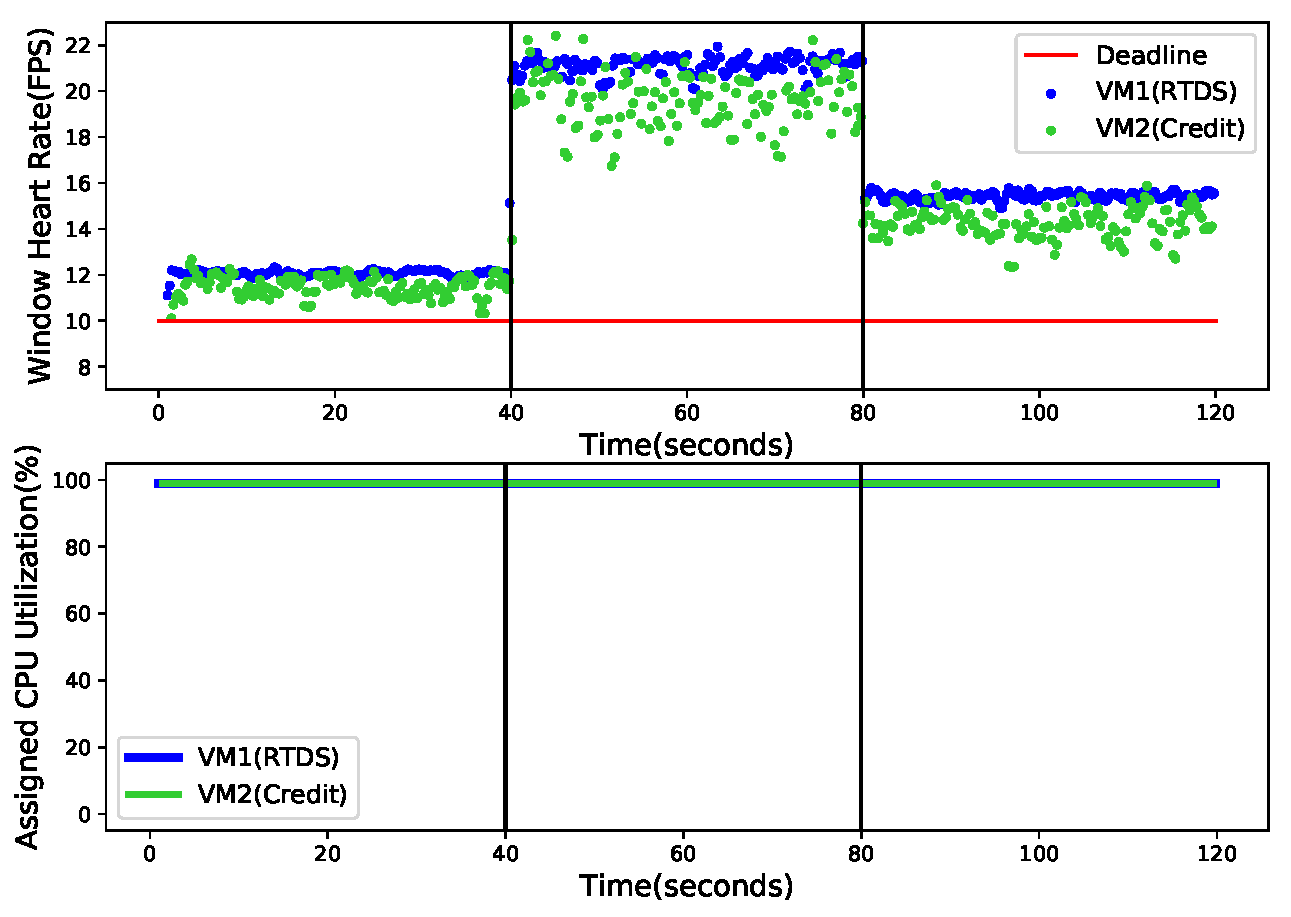
\includegraphics[width=1\linewidth]{images/1vm_static}
\caption{Static Algorithm Result for Experiment 1}
\label{1vm_static}
\end{figure}

\begin{figure}[h!]
\centering
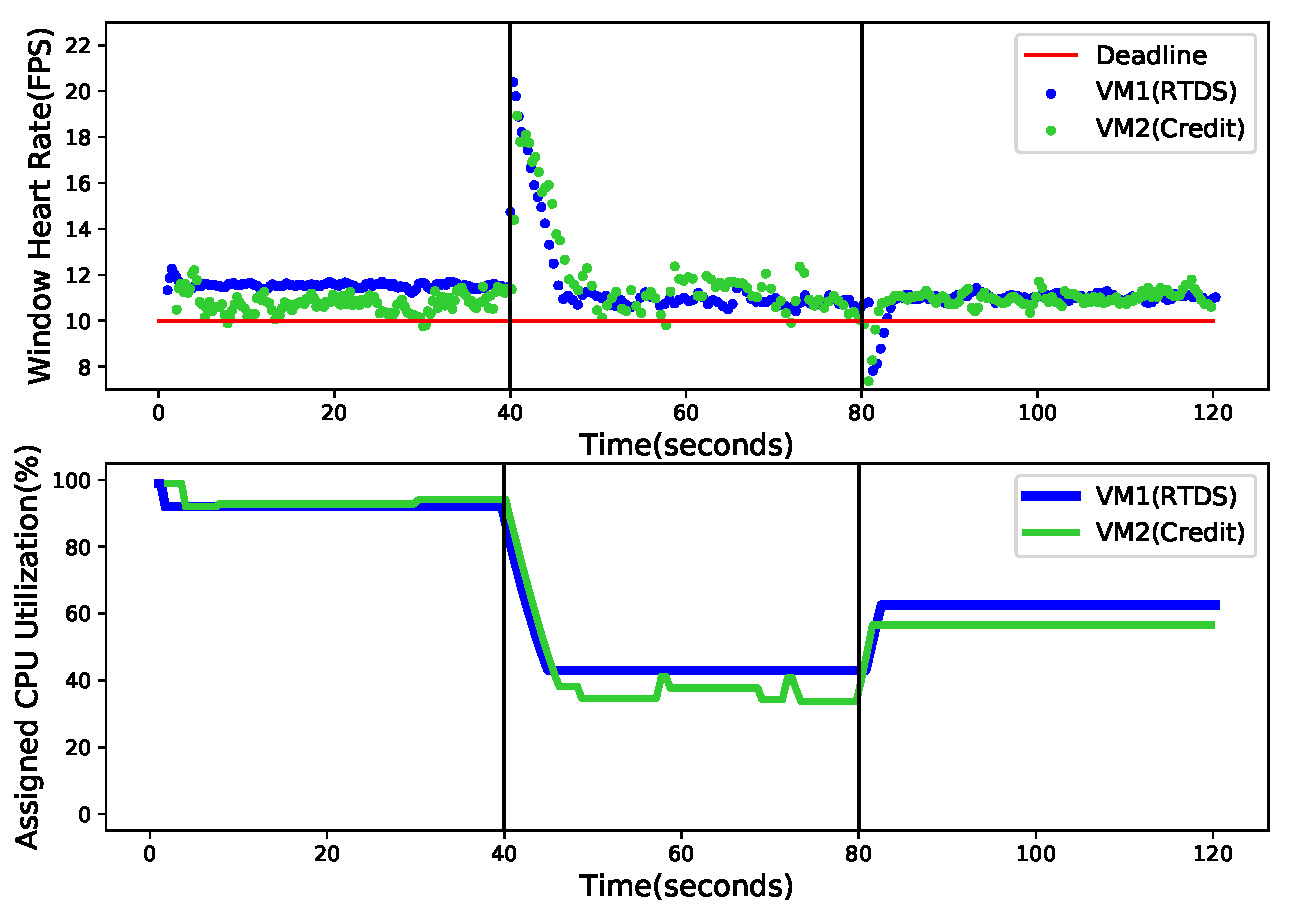
\includegraphics[width=1\linewidth]{images/1vm_aimd}
\caption{AIMD Algorithm Result for Experiment 1}
\label{1vm_aimd}
\end{figure}

\begin{figure}[h!]
\centering
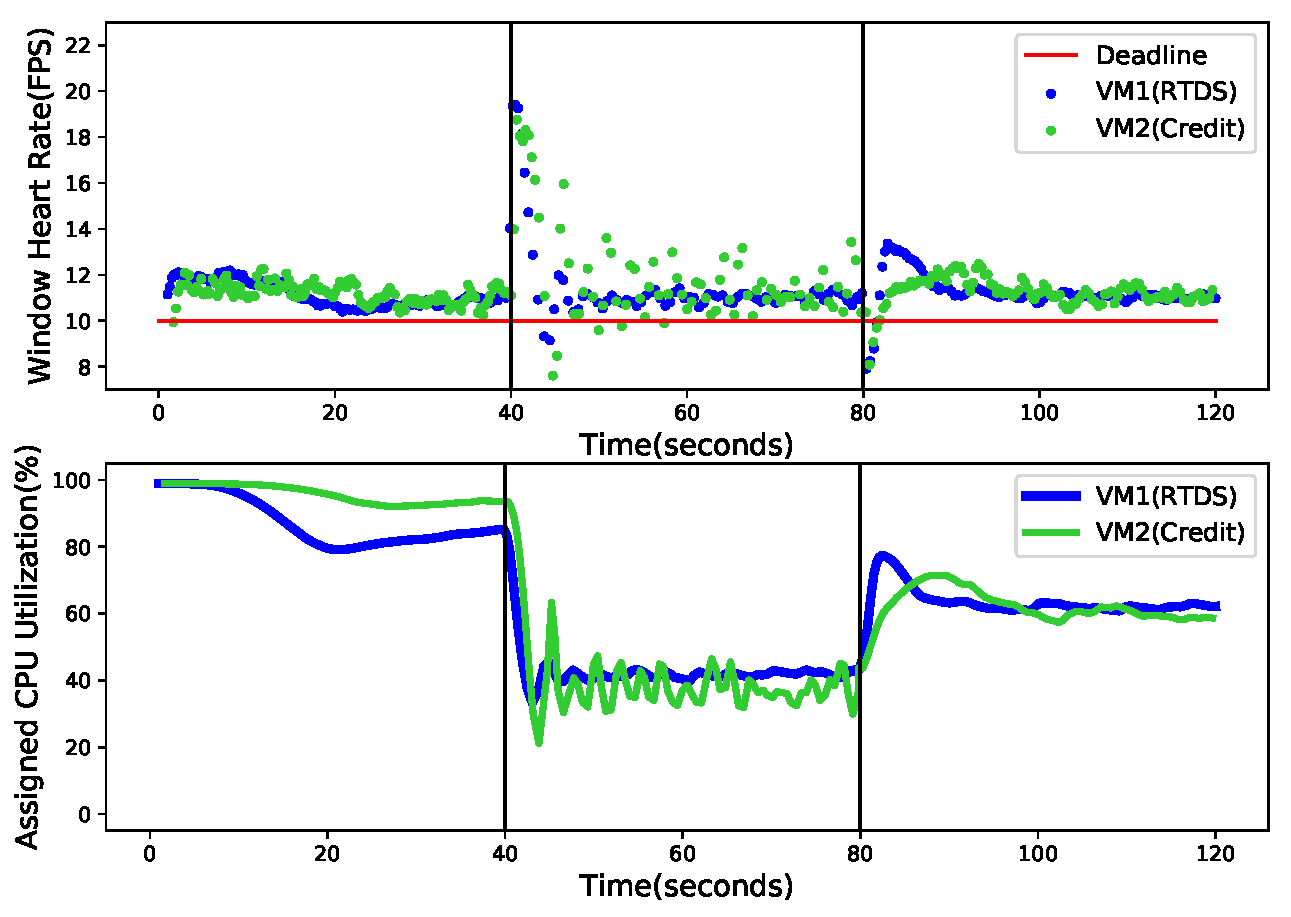
\includegraphics[width=1\linewidth]{images/1vm_apid}
\caption{STPID Algorithm Result for Experiment 1}
\label{1vm_apid}
\end{figure}



\subsubsection*{Result \& Analysis}\hfill\\
\indent The experiment results are shown in figure \ref{1vm_static}, \ref{1vm_aimd} and \ref{1vm_apid}. In these three figures, the first vertical line indicates when the workload is manually changed from heavy to light. The second vertical line indicates when the workload is switched from light to medium. The top subplots show the heart rates, and the bottom subplots show the CPU utilization assignments. For the static allocation results shown in figure \ref{1vm_static}, although no heart rate drops below the deadline (10 FPS) for the entire 120 seconds, CPU resources can be saved without missing deadlines in the light and medium workload regions from 40 to 120 seconds. For the AIMD and STPID results shown in figure \ref{1vm_aimd} and \ref{1vm_apid}, both algorithms are able to lower CPU usage (making resources available for other applications) while keeping heart rates above the deadline and able to raise CPU utilization when deadline miss is detected. 

Figure \ref{1vm_rtds} shows the performance of the AIMD and STPID algorithms when the VM is running under the RTDS scheduler. Figure \ref{1vm_rtds_fps} shows the real-time performance of all three allocations. In figure \ref{1vm_rtds_fps}, in the first 40 seconds, all three allocations are able to meet the deadlines. Despite being under heavy workload in the first 40 seconds, AIMD and STPID are able to save 6.88\% and 11.3\% of CPU utilization respectively as shown in figure \ref{1vm_rtds_cpu}. 

Between 40 to 80 seconds, figure \ref{1vm_rtds_fps} shows that AIMD is still able to maintain perfect real-time performance, but the percentage of heart beats that meet  the deadline for STPID drops slightly to 97.37\% due to overshoot. Since it is under light workload, we can see from figure\ref{1vm_rtds_cpu} that both AIMD and STPID can achieve more than 50\% of CPU utilization savings. 

For the final 80 to 120 seconds shown in figure \ref{1vm_aimd} and \ref{1vm_apid}, the initial switch from light to medium workload causes deadline misses for AIMD and STPID, but both algorithms adjust CPU utilizations based on the feedback and are still able to meet deadlines 96.36\% and 96.49\% of the time as shown in figure \ref{1vm_rtds_fps}. Under medium workload, AIMD and STPID can save more than 35\% CPU utilization as shown in figure \ref{1vm_rtds_cpu}.


Similar performance is observed for the Credit scheduler in figure \ref{1vm_credit}. Even though the Credit scheduler achieves more CPU utilization savings, its real-time performance is worse than the RTDS scheduler. Figure \ref{1vm_static} also shows that the heart rates reported under the RTDS scheduler have less variance compared with the heart rates reported under Credit scheduler. A similar trend is observed when using other resource allocation algorithms as shown in figure \ref{1vm_aimd} and figure \ref{1vm_apid}. 

In this experiment, we show that Pacer can work with VMs that are operating under different PCPU pools and hypervisor schedulers. We also verify that the RTDS scheduler is more suitable for real-time applications than Credit scheduler. From this observation, we use RTDS scheduler as the main hypervisor scheduler for the following two experiments. 








\begin{figure*}[t!]
\centering

\begin{subfigure}{.45\textwidth}
    \centering
    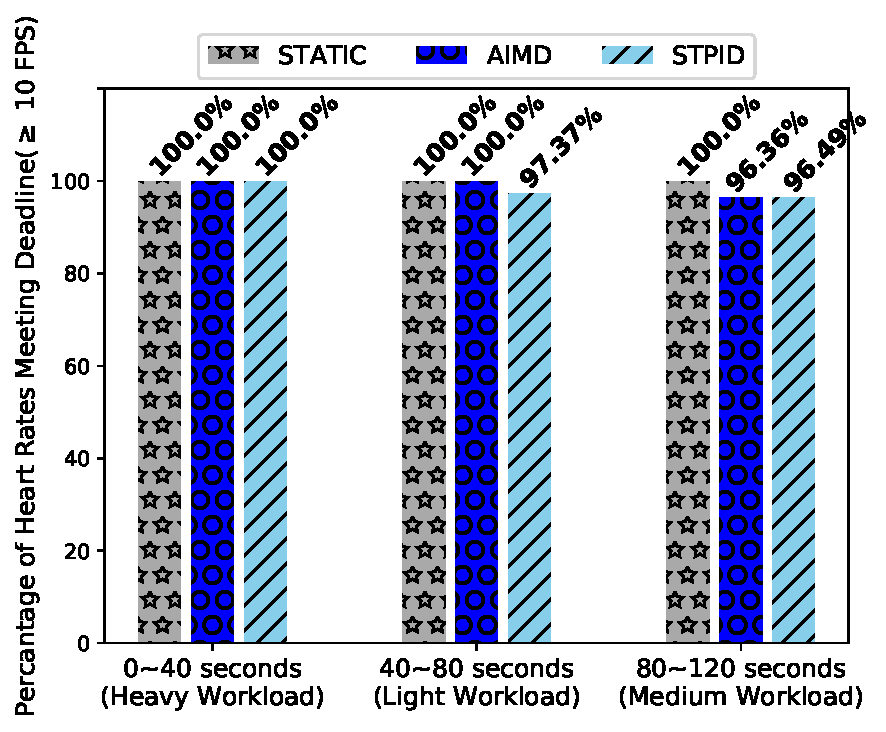
\includegraphics[width=1\linewidth]{images/1vm_rtds_fps}
    \caption{Real-time Performance}
    \label{1vm_rtds_fps}
\end{subfigure}
\begin{subfigure}{.45\textwidth}
    \centering
    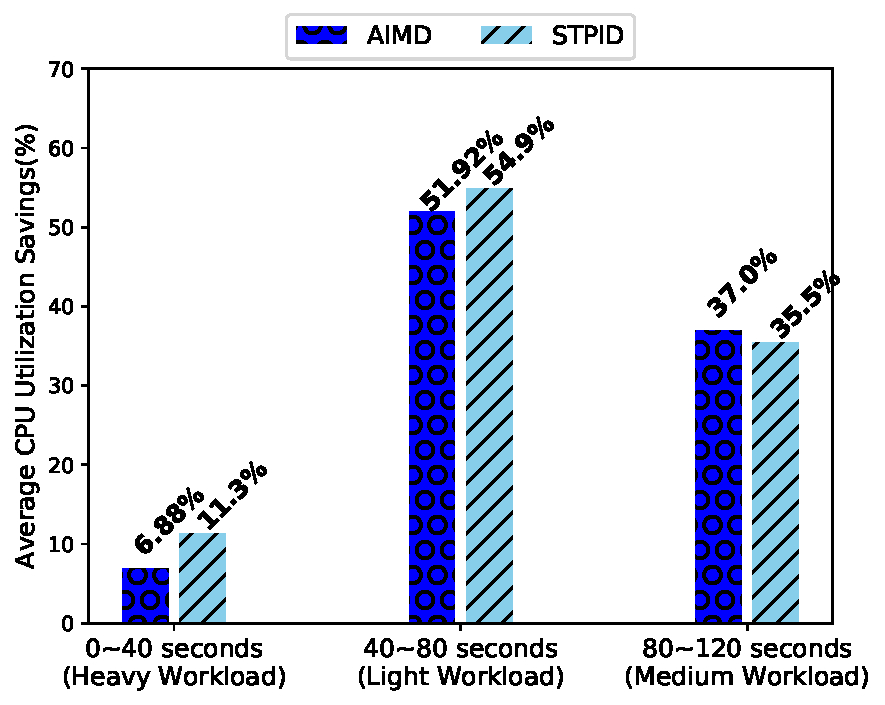
\includegraphics[width=1\linewidth]{images/1vm_rtds_cpu}
    \caption{CPU Utilization Savings}
    \label{1vm_rtds_cpu}
\end{subfigure}%
\captionsetup{justification=centering}
\caption{Performance under RTDS Scheduler}
\label{1vm_rtds}
% \vspace{-0.63cm}
\end{figure*}




\begin{figure*}[t!]
\centering
\begin{subfigure}{.45\textwidth}
    \centering
    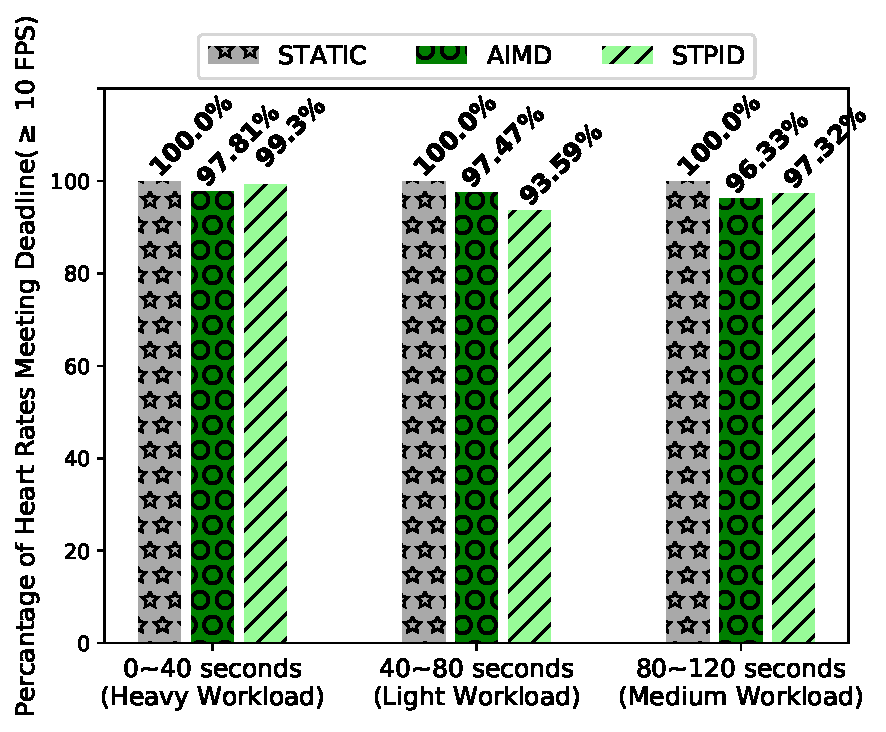
\includegraphics[width=1\linewidth]{images/1vm_credit_fps}
    \caption{Real-time Performance}
    \label{1vm_credit_fps}
\end{subfigure}
\begin{subfigure}{.45\textwidth}
    \centering
    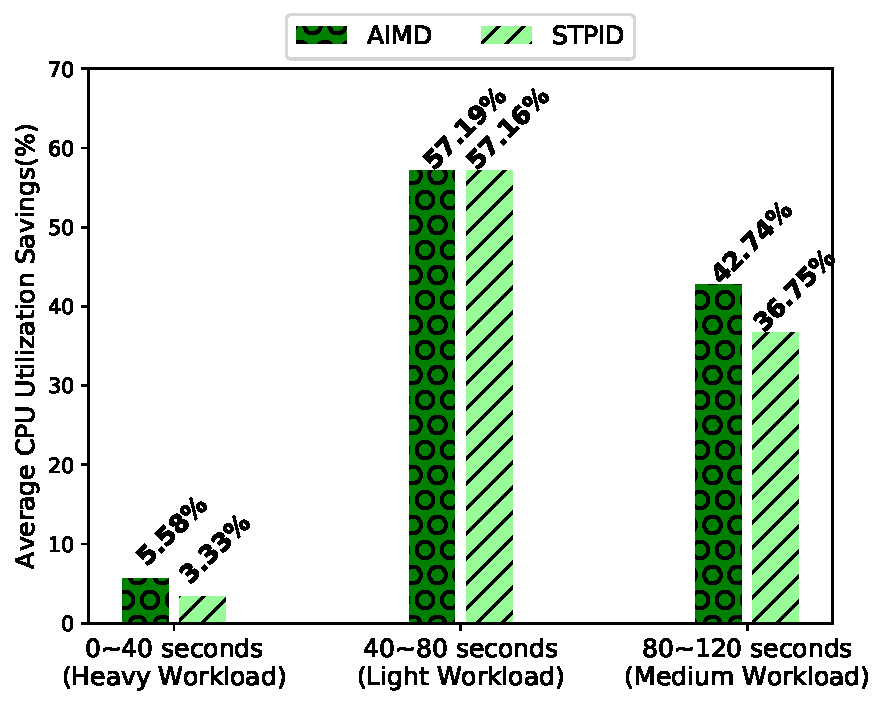
\includegraphics[width=1\linewidth]{images/1vm_credit_cpu}
    \caption{CPU Utilization Savings}
    \label{1vm_credit_cpu}
\end{subfigure}%



\captionsetup{justification=centering}
\caption{Performance under Credit Scheduler}
\label{1vm_credit}
% \vspace{-0.63cm}
\end{figure*}








\subsection{Experiment 2: Monitoring Multiple VMs}

% \hfill \linebreak
In this experiment, we evaluate Pacer's ability to save CPU resources through a simulated video surveillance application and show how the saved CPU resources can be utilized for doing more work.



\subsubsection*{Application}\hfill\\
\indent Three VMs are needed for this experiment. VM1 and VM2 run the real-time application, and VM3 runs a non-real-time application. 
\begin{itemize}
\item Video Surveillance Application: A simulated real-time surveillance application that runs on VM1 and VM2. This soft real-time application reads in video streams and performs object detection. If a person is detected in the current frame, the sampling frequency is switched from low to medium, shifting the workload from light to medium. If no person is detected in the current frame, the sampling frequency is switched to low frequency, shifting the workload from medium to light. Each trial is run for 120 seconds. The waiting time for a person to enter the frame is drawn from an exponential distribution with $\beta=30$ seconds, and the time for a person to stay in the frame is drawn from an exponential distribution with $\beta=15$ seconds. The application exits when the time reaches 120 seconds. To avoid the total CPU resource demands exceeding the system's available resources, video frame size is decreased by 5\% to lower the workload for both low and medium sampling frequency.
\item Matrix Multiplication: A non real-time application that runs on VM3. This application executes continuous matrix multiplication with a matrix size of 500 by 500.
\end{itemize}


\subsubsection*{VM Configuration}\hfill\\
\indent VM1, VM2 and VM3 all run under the same PCPU pool with the RTDS scheduler. To have a fair comparison between static, AIMD and STPID, we first find the static CPU utilization assignment that results in heart rates of 11 FPS for medium sampling frequency. 11 FPS is used because the average of upper and lower bound acceptable heart rates for AIMD and the target heart rate for STPID are both 11 FPS. The resulting static CPU utilization found is 40\%, so VM1 and VM2 are initially assigned with 40\% CPU utilization. VM3 is assigned with the remaining 20\% CPU utilization. The VM configurations are shown in table \ref{exp2setup_table}.

\begin{table}[ht]
\centering
\caption{VM Configurations for Experiment 2}
\label{exp2setup_table}
\begin{tabular}{ @{\hskip6pt}c@{\hskip6pt} c @{\hskip6pt}c@{\hskip6pt}c @{\hskip6pt}c@{\hskip6pt}c }

\hline
\textbf{\phantom{ffffsssss}} & \textbf{\begin{tabular}[c]{@{}c@{}}PCPU\\ Pool\end{tabular}} & \textbf{\begin{tabular}[c]{@{}c@{}}\# of\\ VCPUs\end{tabular}} & \textbf{Scheduler} & \textbf{\begin{tabular}[c]{@{}c@{}}Initial CPU \\ Utilization\end{tabular}} \\ \hline
\rowcolor[HTML]{EFEFEF} 
VM1 & 1 & 5 & RTDS & 40\% \\
\rowcolor[HTML]{EFEFEF} 
VM2 & 1 & 5 & RTDS & 40\% \\
\rowcolor[HTML]{EFEFEF} 
VM3 & 1 & 5 & RTDS & 20\% \\ \hline
\end{tabular}
\end{table}
% \begin{table}[ht]
% \centering
% \caption{VM configurations for Experiment 2}
% \label{exp2setup_table}
% \begin{tabular}{ccccc}
% \hline
% \textbf{} & \textbf{\begin{tabular}[c]{@{}c@{}}PCPU\\ Pool\end{tabular}} & \textbf{\begin{tabular}[c]{@{}c@{}}\# of\\ VCPUs\end{tabular}} & \textbf{Scheduler} & \textbf{\begin{tabular}[c]{@{}c@{}}Initial CPU \\ Utilization\end{tabular}} \\ \hline
% \rowcolor[HTML]{EFEFEF} 
% VM1 & 1 & 5 & RTDS & 40\% \\
% \rowcolor[HTML]{EFEFEF} 
% VM2 & 1 & 5 & RTDS & 40\% \\
% \rowcolor[HTML]{EFEFEF} 
% VM3 & 1 & 5 & RTDS & 20\% \\ \hline
% \end{tabular}
% \end{table}

\subsubsection*{Methodology}\hfill\\
\indent First, we generate two random sequences of timestamps of a person entering and leaving the frame separately for VM1 and VM2. We run the surveillance application in VM1 and VM2 with these two random sequences of frames. As for VM3, for each trial, it starts running the matrix multiplication application when VM1's or VM2's first heartbeat reaches the Pacer resource manager. VM3 stops and reports the number of computations completed when VM1 and VM2 notify the Pacer resource manager that they have finished running their applications. The experiment starts by running VM1, VM2 and VM3 with static CPU resource allocation. The same procedure is then repeated with the AIMD and STPID resource allocation algorithms. For each trial, the resulting heart rates and CPU utilization assignments are recorded for analysis.




\begin{figure}[h!]
\centering
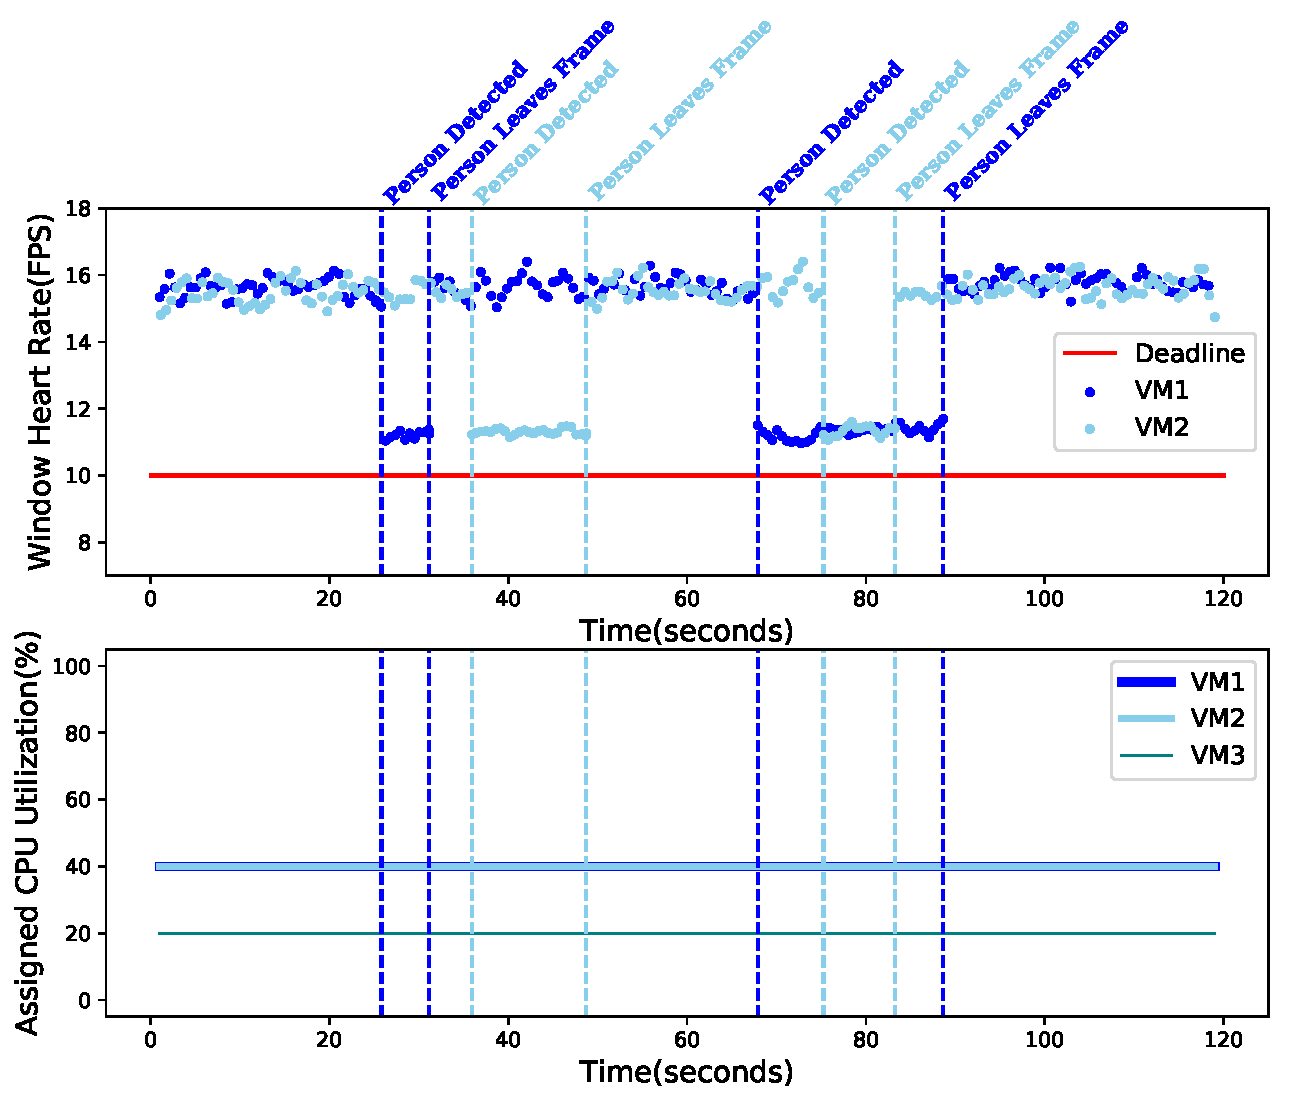
\includegraphics[width=1\linewidth]{images/3vm_static}
\caption{Static Algorithm Result for Experiment 2}
\label{3vm_static}
\end{figure}

\begin{figure}[h!]
\centering
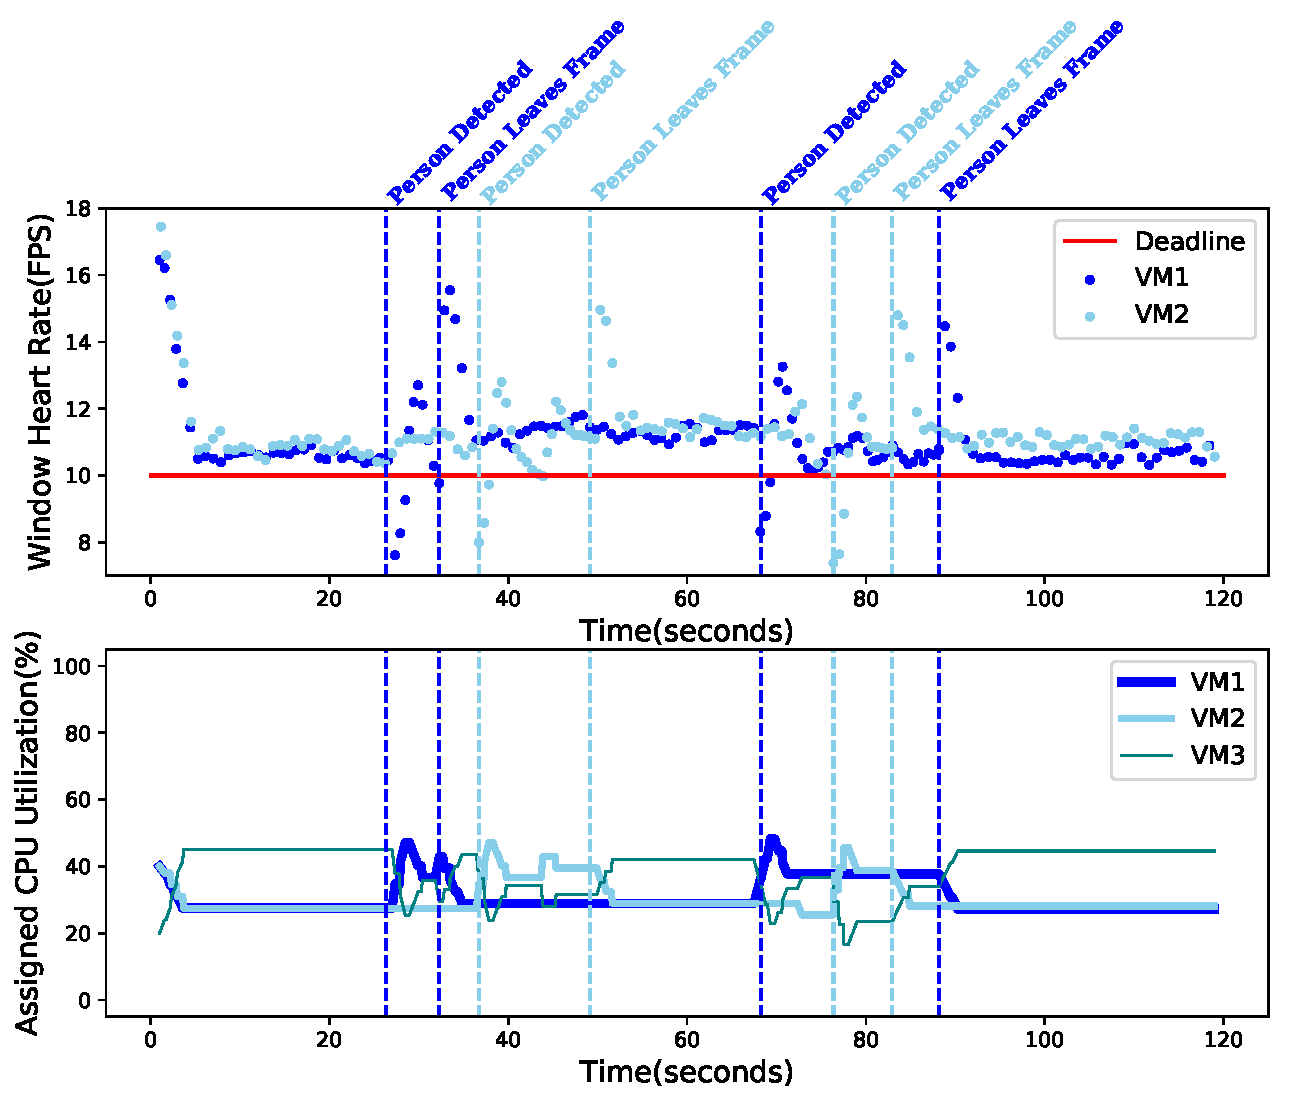
\includegraphics[width=1\linewidth]{images/3vm_aimd}
\caption{AIMD Algorithm Result for Experiment 2}
\label{3vm_aimd}
\end{figure}

\begin{figure}[h!]
\centering
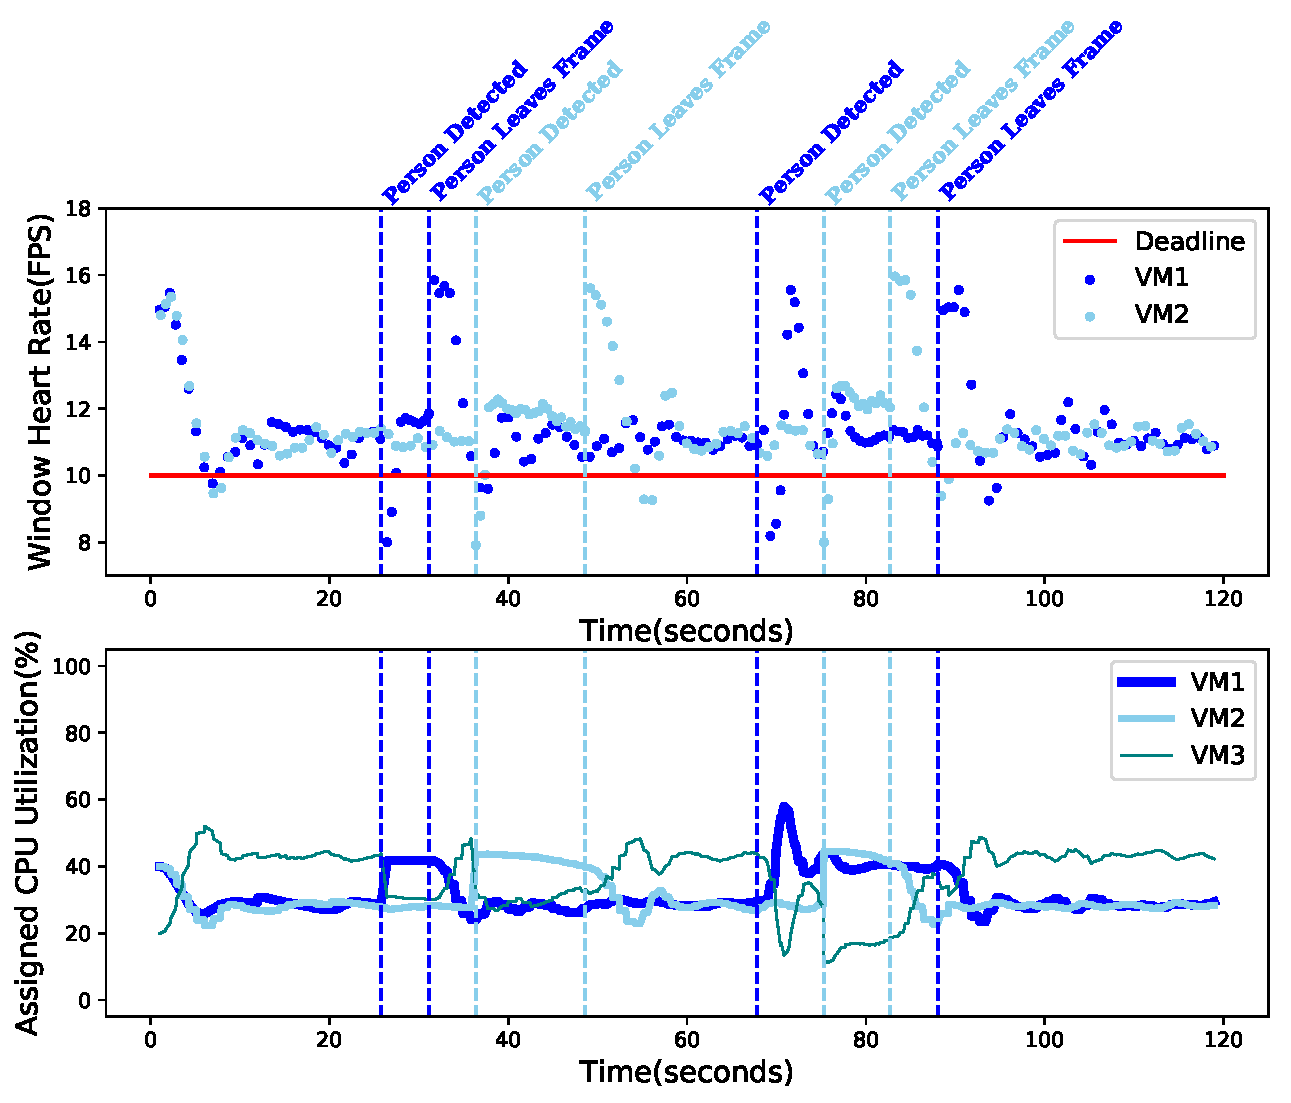
\includegraphics[width=1\linewidth]{images/3vm_apid}
\caption{STPID Algorithm Result for Experiment 2}
\label{3vm_apid}
\end{figure}



\subsubsection*{Result \& Analysis}\hfill\\
\indent The experiment results are shown in figure \ref{3vm_static}, \ref{3vm_aimd} and \ref{3vm_apid}. For these three figures, the vertical lines indicate when a person is detected or when a person leaves the frame. The top subplots show the heart rates, and the bottom subplots show the CPU utilization assignments. For the static allocation shown in figure \ref{3vm_static}, VM1, VM2 and VM3 have constant CPU utilization. As for AIMD and STPID, CPU utilization assigned to VM1, VM2 and VM3 changes based on the heartbeats feedback that reflects workload variation as shown in figure \ref{3vm_aimd} and \ref{3vm_apid}.

Figure \ref{3vm_fps} compares the real-time performance, and figure \ref{matmul} shows the computation counts of VM3 under three different resource allocation algorithms. The static algorithm is able to meet the FPS requirement 100\% of the time, but has the lowest matrix computation count of 743. Under AIMD, VM3 is able to increase the computation count to 1112, a 49.67\% increase compared with static allocation performance, with a cost of less than 5\% of the heart rates missing deadline for both VM1 and VM2. Finally, under STPID, VM3 achieves computation counts of 1064 while more than 93\% of the heart rates meet their deadline for both VMs.

In this experiment, we show that Pacer is able to handle non-deterministic workload changes and save CPU resources to perform more computations.



\begin{figure}[h!]
\centering
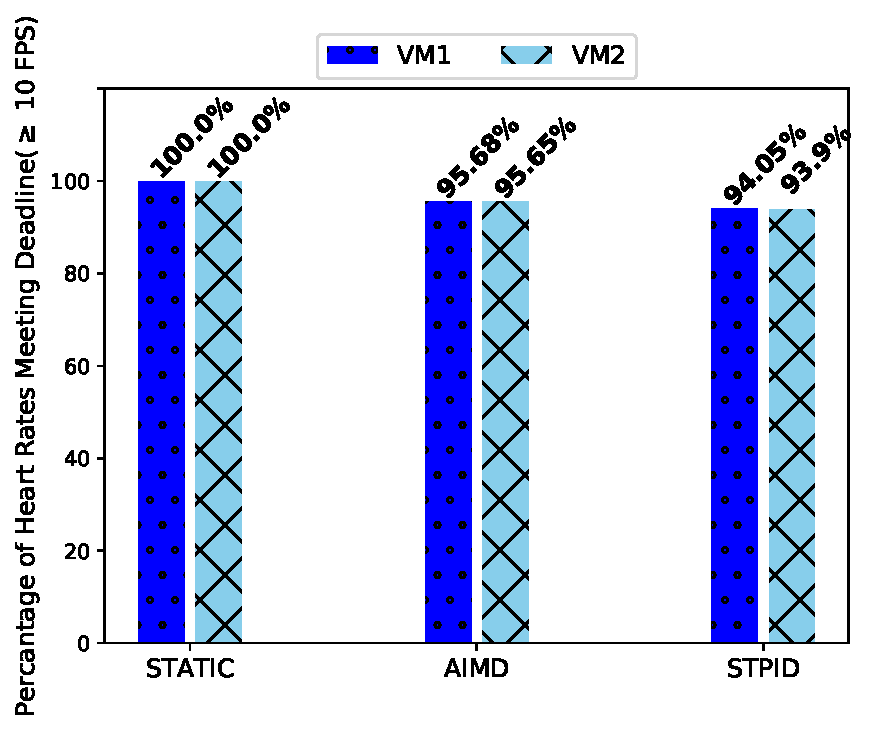
\includegraphics[width=.9\linewidth]{images/3vm_fps}
\caption{Real-time Performance Comparison for Experiment 2}
\label{3vm_fps}
\end{figure}


\begin{figure}[h!]
\centering
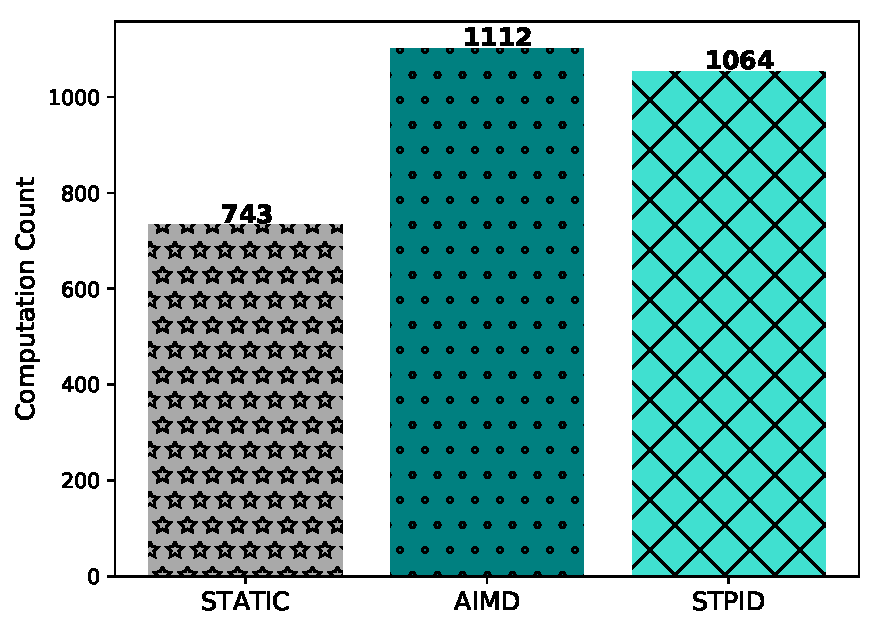
\includegraphics[width=.9\linewidth]{images/matmul}
\caption{VM3 Computation Counts Comparison}
\label{matmul}
\end{figure}







\subsection{Experiment 3: Monitoring VMs in an Oversubscribed System}

In this experiment, we show that Pacer is able to satisfy VMs' soft real-time requirements when static allocation fails to do so. We also demonstrate that Pacer can improve real-time performance when the total resource demands from the VMs exceed the system's available resources.


\subsubsection*{Application}\hfill\\
\indent Both VM1 and VM2 run the same object detection application as in experiment 2 but with deterministic sequence of frames with or without a person present as shown in figure \ref{exp3seq}. Deterministic sequences of frames are used because we want to emphasize how Pacer performs under various system loads. For this experiment, the application runs at medium sampling frequency when a person is not detected in a frame, and switches to high sampling frequency when a person is detected in a frame. To create an overloading scenario, we increase the overall workload by increasing the frame size by 5\%.


\begin{figure}[h!]
\centering
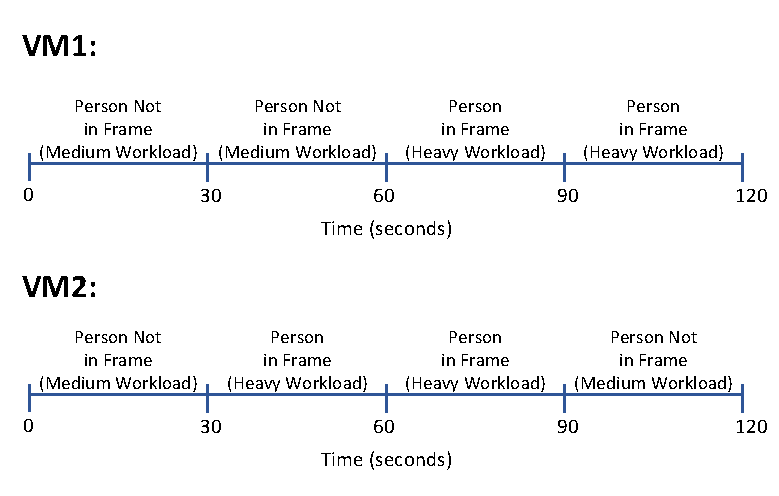
\includegraphics[width=1\linewidth]{images/exp3seq}
\caption{Deterministic Video Frames Sequences for Experiment 3}
\label{exp3seq}
\end{figure}



\subsubsection*{--- VM Configuration}\hfill\\
\indent VM1 and VM2 run in the same PCPU pool. Both VMs are initially assigned with 50\% CPU utilization. The configuration is shown in table \ref{exp3setup_table}.

% \begin{table}[ht]
% \centering
% \caption{Stride Sharing Parameter Configurations}
% \label{strideh}
% \begin{tabular}{@{}|c|c|c|c|@{}}
% \toprule
% \multicolumn{4}{|c|}{\textbf{Stride Sharing}} \\ \midrule
% \begin{tabular}[c]{@{}c@{}}Scheduling \\ Quantum\end{tabular} & 6 seconds& \begin{tabular}[c]{@{}c@{}}Weight\end{tabular} & 1 \\ \bottomrule
% \end{tabular}
% \end{table}




\begin{table}[ht]
\centering
\caption{VM Configurations for Experiment 3}
\label{exp3setup_table}
% \begin{tabular}{ccccc}
\begin{tabular}{ @{\hskip6pt}c@{\hskip6pt} c @{\hskip6pt}c@{\hskip6pt}c @{\hskip6pt}c@{\hskip6pt}c }

\hline
\textbf{\phantom{ffffsssss}} & \textbf{\begin{tabular}[c]{@{}c@{}}PCPU\\ Pool\end{tabular}} & \textbf{\begin{tabular}[c]{@{}c@{}}\# of\\ VCPUs\end{tabular}} & \textbf{Scheduler} & \textbf{\begin{tabular}[c]{@{}c@{}}Initial CPU \\ Utilization\end{tabular}} \\ \hline

% \textbf{} & \textbf{\begin{tabular}[c]{@{}c@{}}PCPU\\ Pool\end{tabular}} & \textbf{\begin{tabular}[c]{@{}c@{}}\# of\\ VCPUs\end{tabular}} & \textbf{Scheduler} & \textbf{\begin{tabular}[c]{@{}c@{}}Initial CPU \\ Utilization\end{tabular}} \\ \hline
\rowcolor[HTML]{EFEFEF} 
VM1 & 1 & 5 & RTDS & 50\% \\
\rowcolor[HTML]{EFEFEF} 
VM2 & 1 & 5 & RTDS & 50\% \\ \hline
\end{tabular}
\end{table}




\subsubsection*{Methodology}\hfill\\
\indent Before each trial, both VMs are configured according to table \ref{exp3setup_table}. The experiment starts with VM1 and VM2 running with static CPU utilization assignments. The same procedure is then repeated with the AIMD and STPID resource allocation algorithms and the stride sharing algorithm. For each trial, resulting heart rates and CPU utilization assignments are recorded for analysis.

\begin{figure}[h!]
\centering
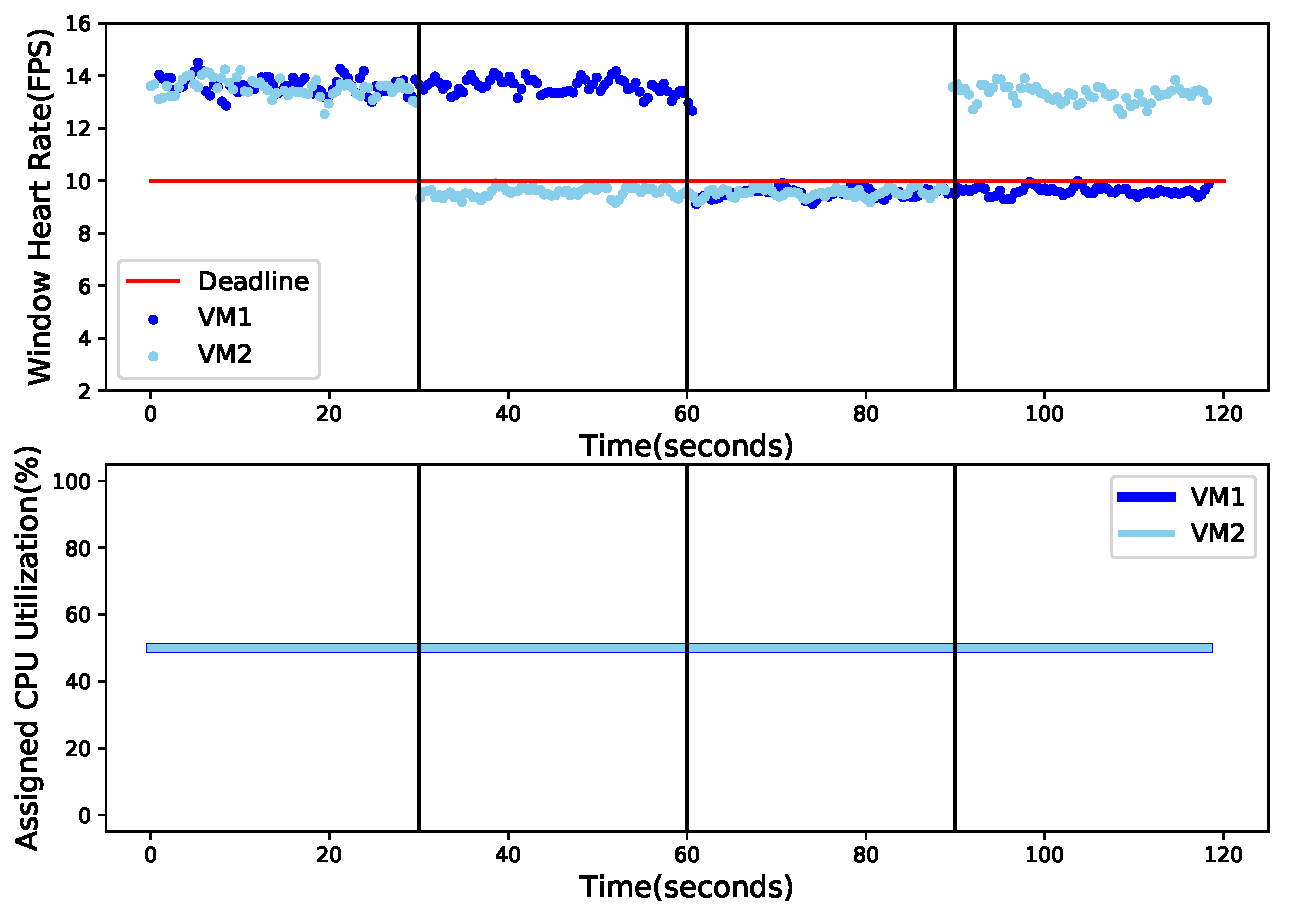
\includegraphics[width=1\linewidth]{images/2vm_static}
\caption{Static Algorithm Result for Experiment 3}
\label{2vm_static}
\end{figure}

\begin{figure}[h!]
\centering
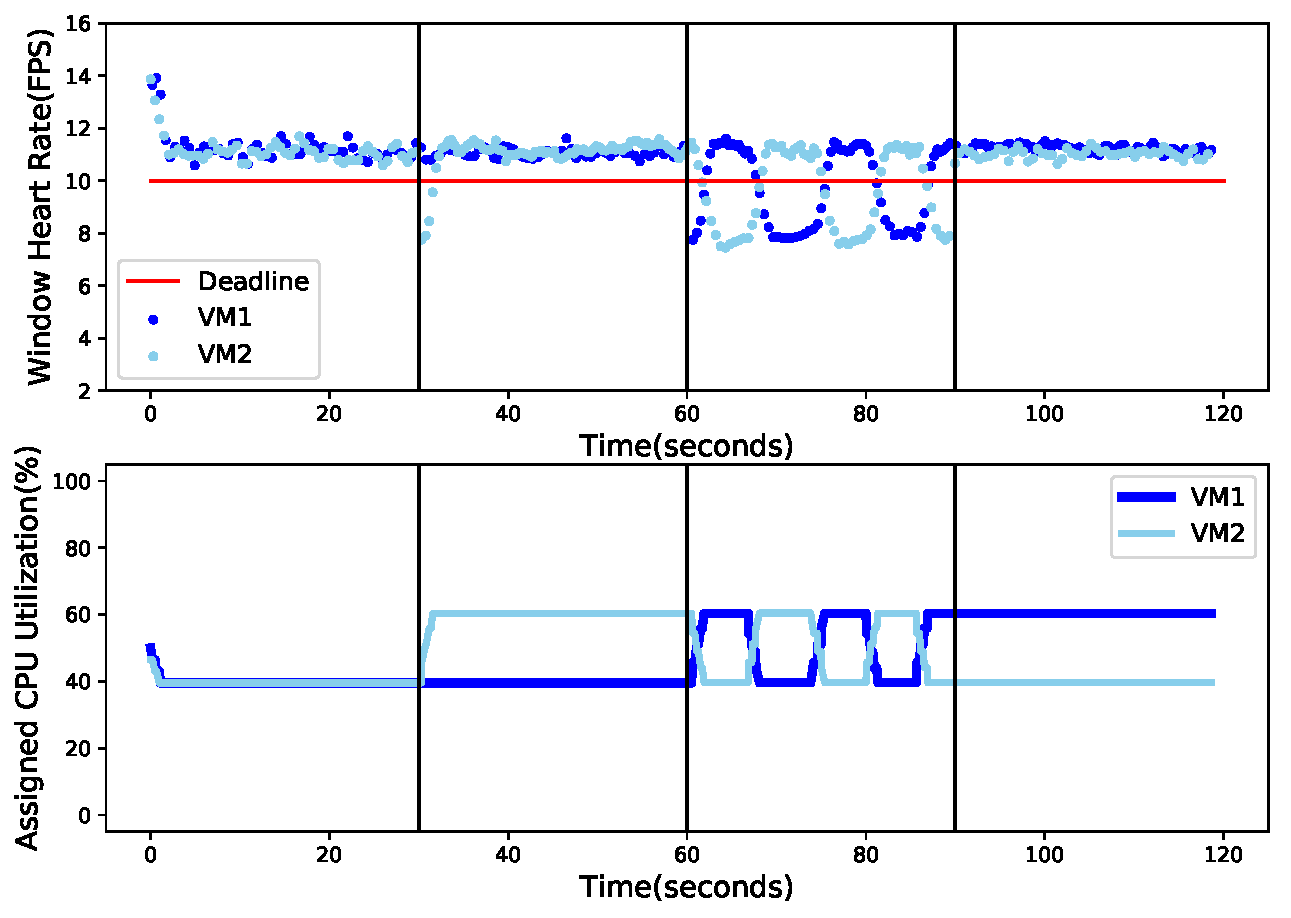
\includegraphics[width=1\linewidth]{images/2vm_aimd}
\caption{AIMD Algorithm Result for Experiment 3}
\label{2vm_aimd}
\end{figure}

\begin{figure}[h!]
\centering
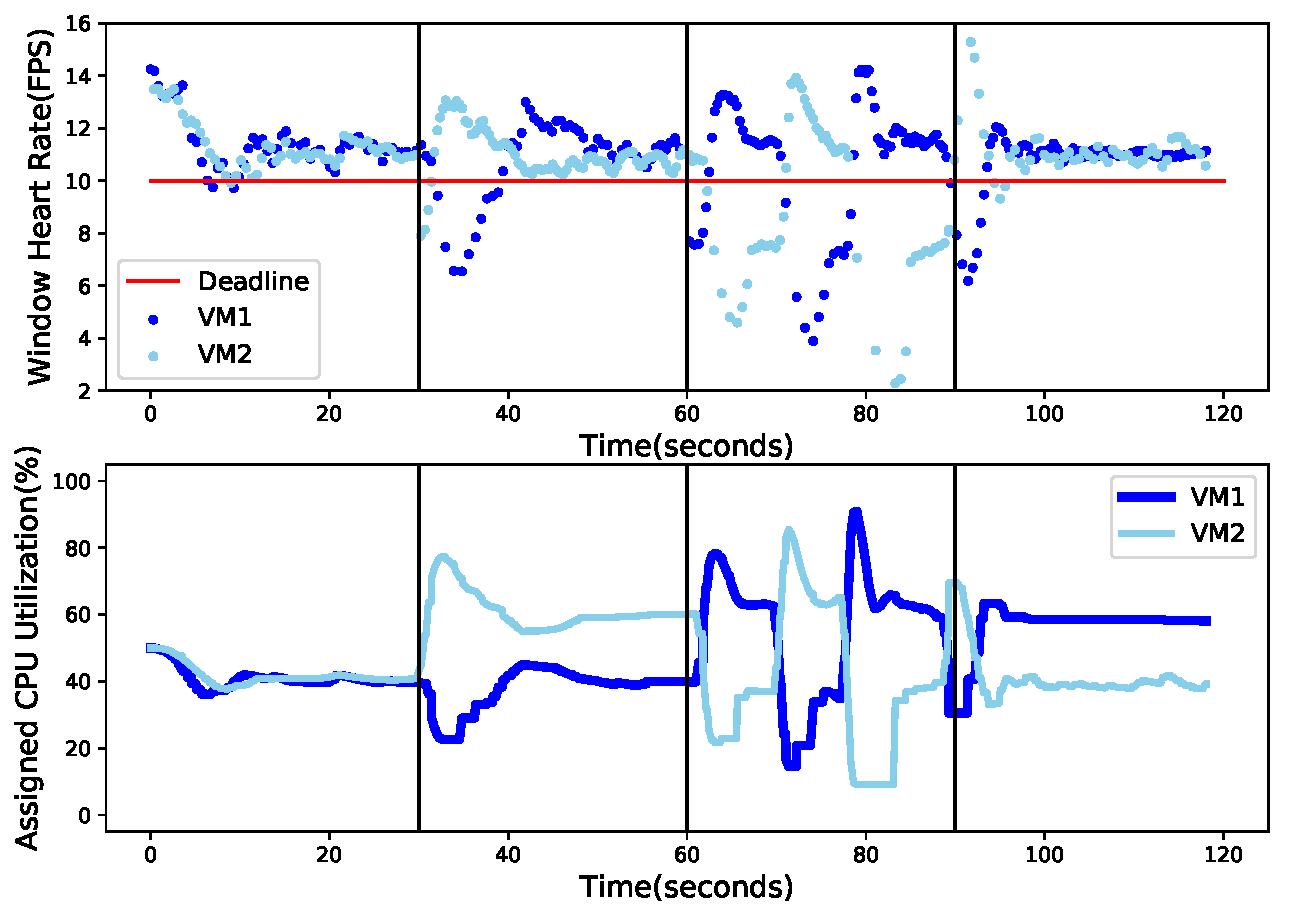
\includegraphics[width=1\linewidth]{images/2vm_apid}
\caption{STPID Algorithm Result for Experiment 3}
\label{2vm_apid}
\end{figure}


\begin{figure*}[ht!]
\centering
\begin{subfigure}{.45\textwidth}
    \centering
    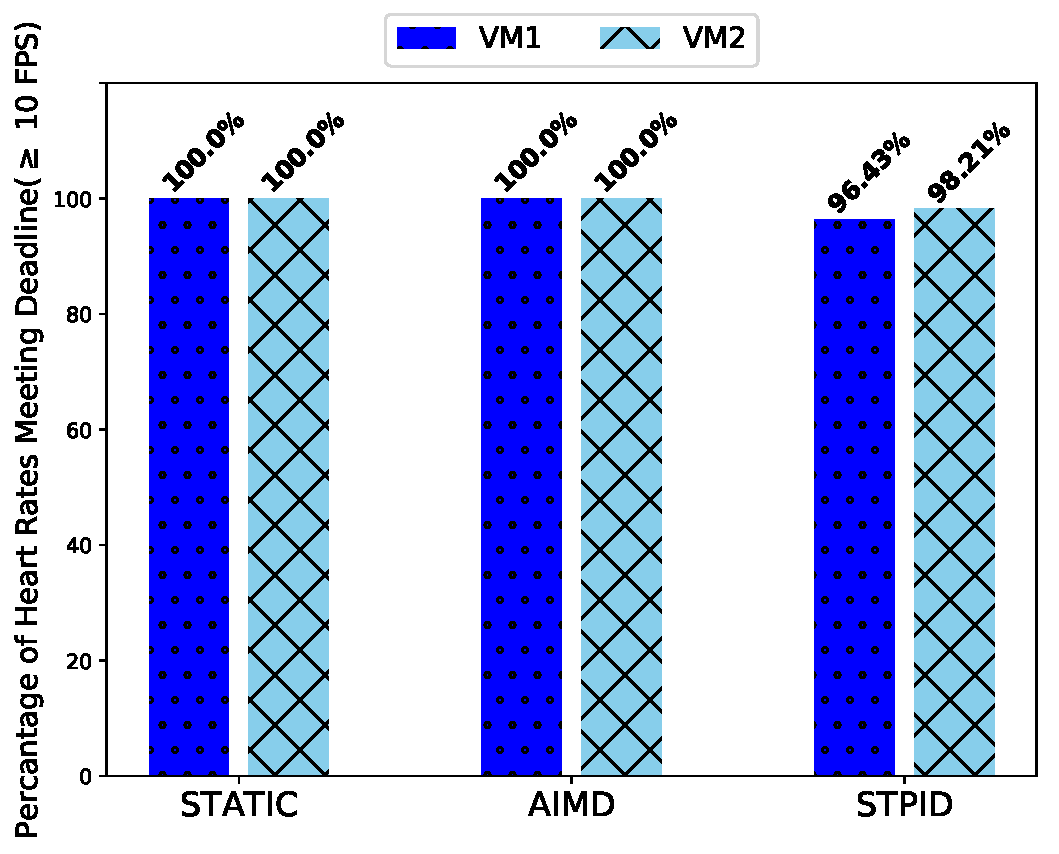
\includegraphics[width=1\linewidth]{images/2vm_r1} 
    \captionsetup{justification=centering}
    \caption{0$\sim$30 seconds\\VM1:Medium Workload\\VM2:Medium Workload}
    \label{2vm_r1}
\end{subfigure}
\begin{subfigure}{.45\textwidth}
    \centering
    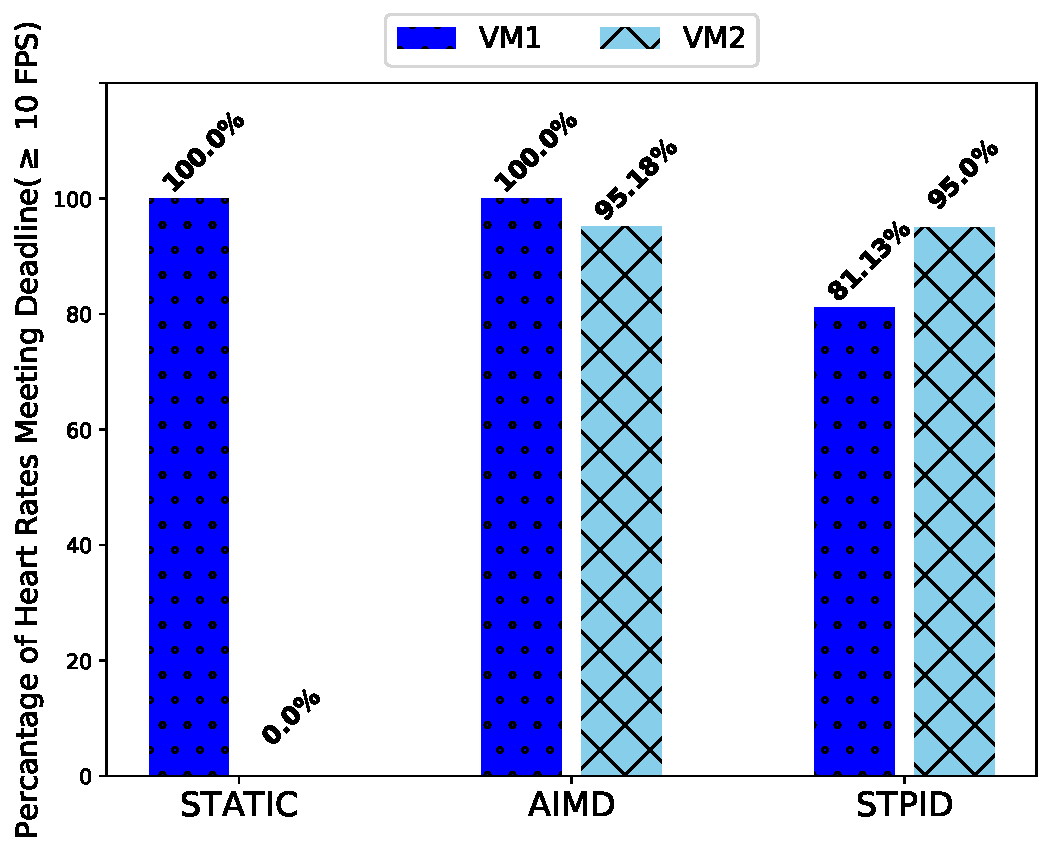
\includegraphics[width=1\linewidth]{images/2vm_r2} 
    \captionsetup{justification=centering}

    \caption{30$\sim$60 seconds\\VM1:Medium Workload \\VM2:Heavy Workload} 
    \label{2vm_r2}
\end{subfigure}%

\begin{subfigure}{.45\textwidth}
    \centering
    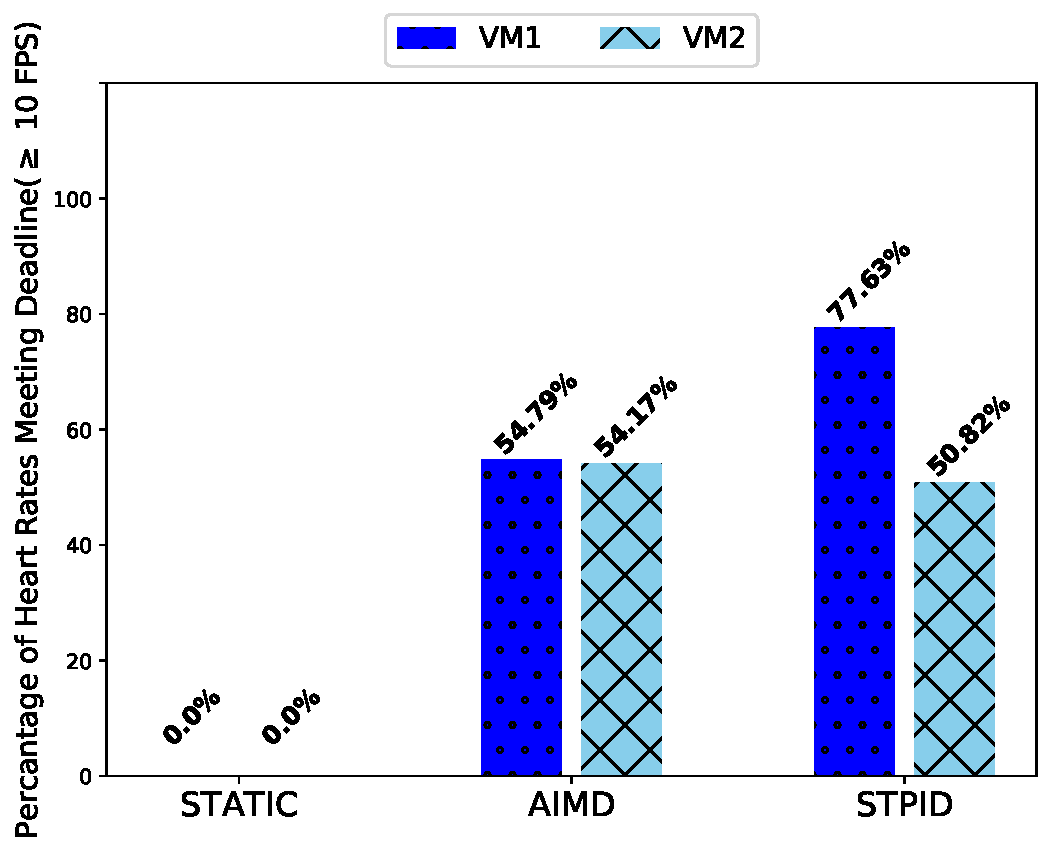
\includegraphics[width=1\linewidth]{images/2vm_r3} 
    \captionsetup{justification=centering}

 \caption{60$\sim$90 seconds\\VM1:Heavy Workload \\VM2:Heavy Workload} 

    \label{2vm_r3}
\end{subfigure}
\begin{subfigure}{.45\textwidth}
    \centering
    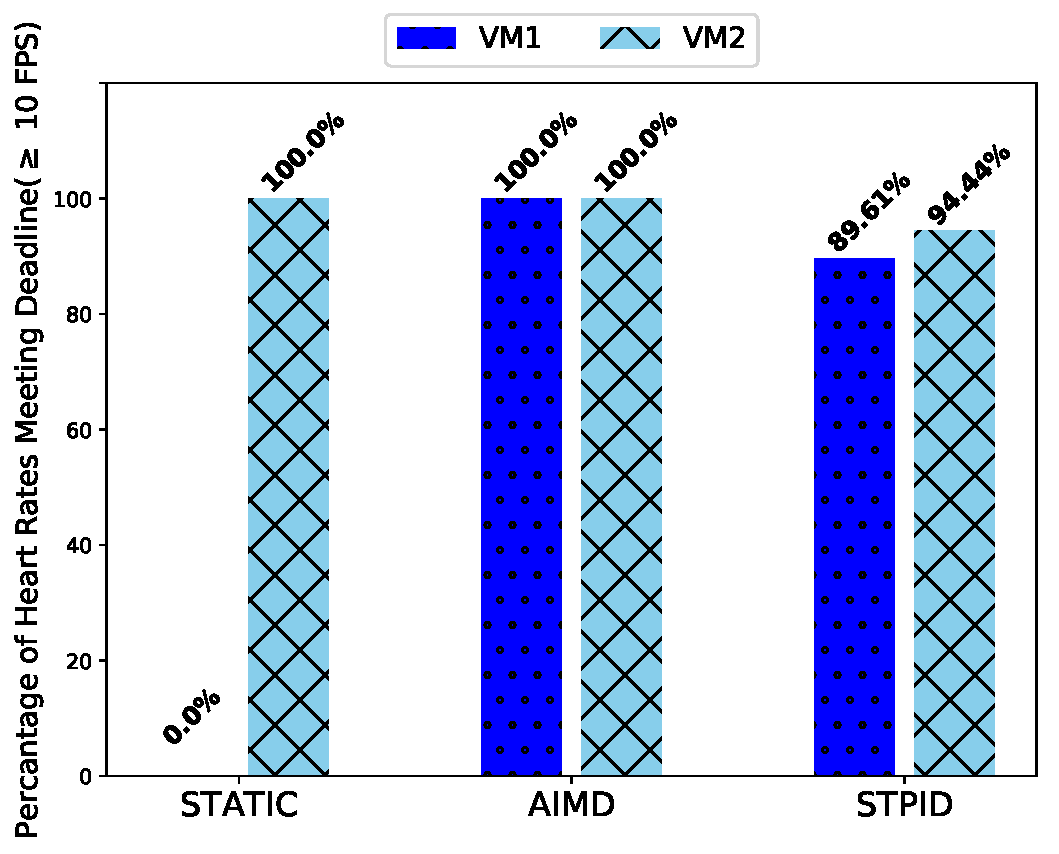
\includegraphics[width=1\linewidth]{images/2vm_r4} 
    \captionsetup{justification=centering}
 \caption{90$\sim$120 seconds\\VM1:Heavy Workload \\VM2:Medium Workload} 
    \label{2vm_r4}
\end{subfigure}%

\captionsetup{justification=centering}
\caption{Real-time Performance Comparison in an Oversubscribed System}
\label{2vm_fps}
\end{figure*}

\subsubsection*{Result \& Analysis}\hfill\\
  \indent The recorded CPU utilization assignments and heart rates data are shown in figure \ref{2vm_static}, \ref{2vm_aimd} and \ref{2vm_apid}. For these three figures, the first vertical line indicates when the workload for VM2 is switched from medium to heavy. The second vertical line indicates when the workload for VM1 is switched from medium to heavy, and the last vertical line indicates when the workload for VM2 is switched from heavy to medium. The top subplots show the heart rates and the bottom subplot show the CPU utilization assignments.
  
The real-time performance comparison of static, AIMD and STPID is shown in figure \ref{2vm_fps}. In the first 30 seconds, both VM1 and VM2 run under medium workload. Figure \ref{2vm_r1} shows that static and AIMD have no deadline misses. STPID has less than 4\% missed deadlines due to overshoot as shown in figure \ref{2vm_apid}.

Figure \ref{2vm_r2} shows the real-time performance comparison from 30 to 60 seconds when VM2 switches to heavy workload mode. Under static allocation, none of the VM2's heart rates can meet the deadline, but with AIMD, VM2's heart rates can meet the deadline 95.18\% of the time while enabling VM1' heart rates to meet all deadlines. STPID has a slightly worse real-time performance than AIMD but is still able to keep VM1's and VM2's heart rate under the deadline 81.13\% and 95.0\% of the time respectively.

System overloading occurs between 60 and 90 seconds when both VMs are in heavy workload mode. Figure \ref{2vm_r3} shows that all heart rates from both VMs miss their deadlines under static allocation. With a scheduling quantum of 6 seconds and setting equal stride values for both VMs, stride sharing is able improve heart rates for both VMs to meet deadlines more than 50\% of the time with AIMD and STPID as shown in figure \ref{2vm_r3}.

Figure \ref{2vm_r4} shows the real-time performance comparison between 90 and 120 seconds when VM2 switches to medium workload and VM1 remains in heavy workload mode. Similar behavior is observed in figure \ref{2vm_r2} but with VM1 missing all the deadlines under static allocation. On the other hand, AIMD is able to have both VMs meet deadlines 100\% of the time, as shown in figure \ref{2vm_r4}. STPID has a slightly worse real-time performance than AIMD but still able to meet VM1's and VM2's heart rate deadlines 89.61\% and 94.44\% of the time respectively.

In this experiment, VM1's and VM2's real-time performance benefit from the Pacer dynamic CPU resource allocation. On the contrary, all the deadlines are missed for the VM running the heavier workload without Pacer. We also shows that stride sharing can improve real-time performance when all deadlines are missed under an overloaded system with static allocation.


